\documentclass[11pt]{article}

\usepackage[french, english]{babel}

\usepackage[T1]{fontenc}

\usepackage{amsfonts}
\usepackage{amsmath}
\usepackage{amssymb}

\usepackage{graphicx}
\usepackage{multirow}
\usepackage{multicol}
\usepackage{xcolor}
\usepackage[shortlabels]{enumitem}

\usepackage[margin=2cm]{geometry}

\usepackage{mathtools}
\usepackage{siunitx}
\usepackage{braket}

\usepackage{listings}

\usepackage{tikz}
\usetikzlibrary{shapes.geometric, arrows.meta, positioning}

\tikzstyle{block} = [rectangle, rounded corners, minimum width=4cm, minimum height=1cm,
text centered, draw=black, fill=blue!10]
\tikzstyle{process} = [rectangle, rounded corners, minimum width=5cm, minimum height=1cm,
text centered, draw=black, fill=green!10]
\tikzstyle{io} = [trapezium, trapezium left angle=70, trapezium right angle=110,
minimum width=4cm, minimum height=1cm, text centered, draw=black, fill=orange!15]
\tikzstyle{decision} = [diamond, aspect=2, draw=black, fill=yellow!15, text centered]
\tikzstyle{arrow} = [thick, ->, >=Stealth]

\renewcommand\lstlistingname{Code Python}

\lstset{frame=tb,
  language=Python,
  numbers=left,
  stepnumber=1,
  aboveskip=3mm,
  belowskip=3mm,
  showstringspaces=false,
  columns=flexible,
  basicstyle={\small\ttfamily},
%   numbers=none,
  numberstyle=\tiny\color{gray},
  keywordstyle=\color{blue},
  commentstyle=\color{paired2b},
  stringstyle=\color{paired3b},
  breaklines=true,
  breakatwhitespace=true,
  tabsize=1,
  frame=single,
%   showtabs=false,
}

\newcounter{questioncounter}
\newenvironment{question}[1]{
\refstepcounter{questioncounter}
\noindent\rule{0.05\textwidth}{1pt}\,\,\raisebox{-.3\ht\strutbox}{\textbf{Question \thequestioncounter : #1}}\,\,\hrulefill\par\vspace{0.4cm}
}{\par}

\begin{document}

\begin{multicols}{2}
  \section{\underline{Produit tensoriel}}

  \subsection{Produit scalaire entre deux spins}
  $\braket{\uparrow|\downarrow}=1$,
  $\braket{\uparrow|\downarrow}=0$,
  $\braket{\downarrow|\uparrow}=0$,
  $\braket{\downarrow|\downarrow}=1$,
  \subsection{Mesure de 2 spins}
  $\ket{\uparrow}\otimes\ket{\uparrow} = \ket{\uparrow}\otimes\frac{1}{\sqrt{2}}[\ket{\uparrow}+\ket{\uparrow}] = \frac{\ket{\uparrow\uparrow}+\ket{\uparrow\downarrow}}{\sqrt{2}}$\\
  $\ket{\uparrow}\otimes\ket{\downarrow} = \ket{\uparrow}\otimes\frac{1}{\sqrt{2}}[\ket{\uparrow}-\ket{\downarrow}] = \frac{\ket{\uparrow\uparrow}-\ket{\uparrow\downarrow}}{\sqrt{2}}$\\
  $\ket{\downarrow}\otimes\ket{\uparrow} = \ket{\downarrow}\otimes\frac{1}{\sqrt{2}}[\ket{\uparrow}+\ket{\downarrow}] = \frac{\ket{\downarrow\uparrow}+\ket{\downarrow\downarrow}}{\sqrt{2}}$\\
  $\ket{\downarrow}\otimes\ket{\downarrow} = \ket{\downarrow}\otimes\frac{1}{\sqrt{2}}[\ket{\uparrow}-\ket{\downarrow}] = \frac{\ket{\downarrow\uparrow}-\ket{\downarrow\downarrow}}{\sqrt{2}}$\\

  \subsection{Quelques définitions et propriétés}
  $\ket{a}\otimes\ket{b} = \ket{a}\ket{b} = \ket{ab}$\\
  $(\alpha\ket{a}+\beta\ket{a'})\otimes\ket{b} = \alpha\ket{a}\otimes\ket{b} + \beta\ket{a'}\otimes\ket{b}$\\
  $\bra{a}\otimes\bra{b} = \bra{ab}$\\
  $\braket{ab|a'b'} = \braket{a|a'}\braket{b|b'}$\\

  \section{\underline{Oscillateur harmonique}}
  \subsection{Quelques aides}
  $[a,a]=[a^\dagger,a^\dagger]=0$,\\
  $[a,a^\dagger] = 1$,\\
  $N=a^{\dagger}a$,\\
  $aa^\dagger = a^{\dagger}a$,\\ 
  $aa^\dagger = 1+a^{\dagger}a = 1 + N$
  \subsection{Petit résumé}
  Hamiltonien : $\hat{H}=\frac{{\hat{p}^2}}{2m}+\frac{1}{2}m\omega^2\hat{x}^2$\\
  Énergies : $\hbar\omega\bigg(n + \frac{1}{2}\bigg)$\\
  Opérateurs d'annihilation et de création : $\hat{a}$ et $\hat{a^\dagger}=\sqrt{\frac{m\omega}{2\hbar}}\hat{x}\pm\frac{i}{\sqrt{2m\omega\hbar}}\hat{p}$ respectivement\\

  \section{\underline{Système de spins}}
  (Truc : Sers-toi intelligeament de la sphère de Bloch pour éviter de faire de grosse intégrales.)\\
  On remarque que le spin ne change qu'aux instants où un pulse agit, pas entre.\\
  Le système est conservatif si l'hamiltonien ne dépend pas du temps.\\
  L'évolution dans ls temps se fait en apppliquant la phase globale $e^{\frac{iH_\pm t}{\hbar}}$
  Les spins sont toujours par
  \subsection{Rappel : Diagonalisation de matrice}
  $det(A-\lambda I) = 0$\\
  $\implies(a-\lambda)(d-\lambda)-bc=0$\\
  $\implies\lambda^2-(a+d)\lambda+(ad-bc)=0$
  
  \section{\underline{Propriétés générales}}
  Un observable est $\hat{A^\dagger} = A$\\
  $\hat{A}\ket{a}=a\ket{a}$\\
  Valeur moyenne : $\braket{A}_\psi = \braket{\psi|A|\psi}$\\
  Probabilité : $P(a)=|\braket{a|\psi}|^2$\\
  Commutateur : $[\hat{A},\hat{B}] = \hat{A}\hat{B}-\hat{B}\hat{A}$\\
  Relation incertitude : $\Delta A\Delta B \geq \frac{1}{2}|\braket{[\hat{A},\hat{B}]}|$\\
  Valeur moyenne : $\braket{A}(t)=\braket{\psi|A|\psi}$\\
  Projection d'état : $\braket{e_i|\psi}$ où $e_i$ est un état propre d'une base othonormée.\\


\end{multicols}

\section{\underline{Annexe}}
\begin{figure}[h!]
  \centering
  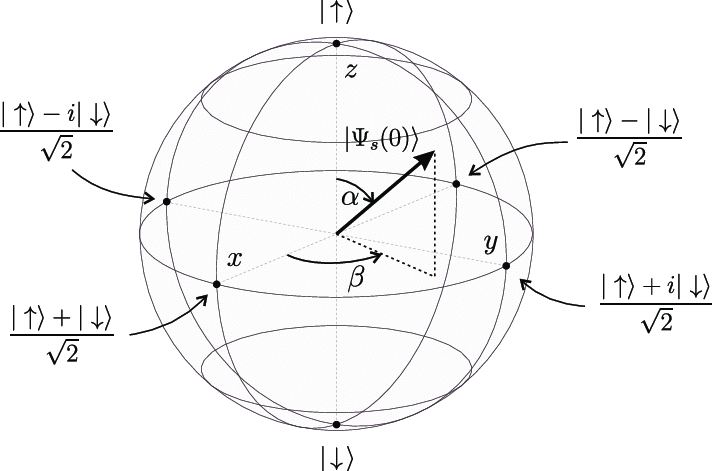
\includegraphics[width=0.5\textwidth]{bloch.jpg}
  \caption{Spins et leur décomposition}
  \label{fig:Figure 1}
\end{figure}

\end{document}